\documentclass[12pt, oneside]{article}
\usepackage[letterpaper, margin=1in, headsep=0.5in, left=0.3in, right=2.5in]{geometry}
\usepackage[english]{babel}
\usepackage[utf8]{inputenc}
\usepackage{amsmath}
\usepackage{amsfonts}
\usepackage{amssymb}
\usepackage{tikz}
\usepackage{yhmath}
\usetikzlibrary{quotes, angles}
\usepackage{graphicx}
\usepackage{enumitem}
\usepackage{multicol}

\newif\ifmeta
\metatrue %print standards and topics tags

\title{Regents Geometry}
\author{Chris Huson}
\date{May 2022}

\usepackage{fancyhdr}
\pagestyle{fancy}
\fancyhf{}
\renewcommand{\headrulewidth}{0pt} % disable the underline of the header
\raggedbottom

%\fancyhead[LE]{\thepage}
\fancyhead[RO]{Name:}
\fancyhead[LO]{BECA / Dr. Huson / Geometry Regents - Problem Bank}
\cfoot{\thepage}

\begin{document}
\subsubsection*{Regents January 2020}
\begin{enumerate}[itemsep=0.5cm]
\item In the diagram below, $\overline{FAD} \parallel \overline{EHC}$, and $\overline{ABH}$ and $\overline{BC}$ are drawn.
\begin{center}
  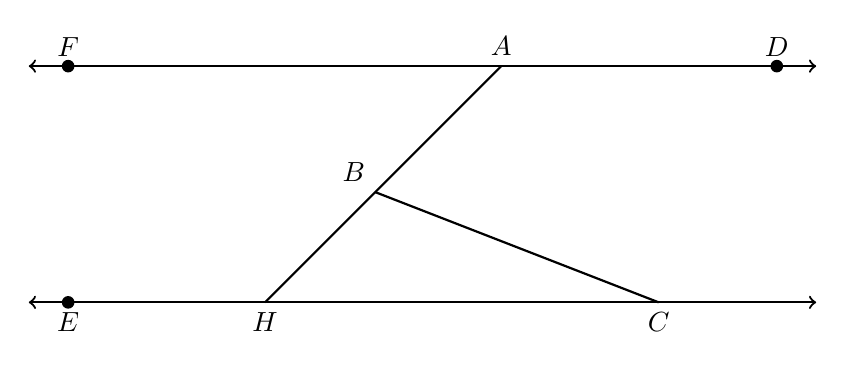
\begin{tikzpicture}[scale=1]
    \draw [thick, <->] (0,0)--(10,0);
    \draw [thick, <->] (0,3)--(10,3);
    \draw [thick] (3,0)node[below]{$H$}--(6,3)node[above]{$A$};
    \draw [thick] (4.4,1.4)node[above left]{$B$}--(8,0)node[below]{$C$};
    \fill (0.5,0) circle [radius=0.08]node[below]{$E$};
    \fill (0.5,3) circle [radius=0.08]node[above]{$F$};
    \fill (9.5,3) circle [radius=0.08]node[above]{$D$};
  \end{tikzpicture}
  \end{center}
If $m\angle FAB = 48^\circ$ and $m\angle ECB = 18^\circ$, what is $m\angle ABC$?
\begin{multicols}{2}
  \begin{enumerate}
    \item $18^\circ$
    \item $48^\circ$
    \item $66^\circ$
    \item $114^\circ$
  \end{enumerate}
\end{multicols}

\item A cone has a volume of $108\pi$ and a base diameter of 12. What is the
height of the cone?

\item The endpoints of directed line segment $PQ$ have coordinates of
$P(-7,-5)$ and $Q(5,3)$. What are the coordinates of point $A$, on $\overline{PQ}$,
that divide $\overline{PQ}$ into a ratio of 1:3?

\item Jaden is comparing two cones. The radius of the base of cone A is
twice as large as the radius of the base of cone B. The height of cone
B is twice the height of cone A. The volume of cone A is
\begin{enumerate}
  \item twice the volume of cone $B$
  \item four times the volume of cone $B$
  \item equal to the volume of cone $B$
  \item equal to half the volume of cone $B$
\end{enumerate}

\item A regular hexagon is rotated about its center. Which degree measure will carry the regular hexagon onto itself? 
\begin{multicols}{2}
  \begin{enumerate}
    \item $45^\circ$
    \item $90^\circ$
    \item $120^\circ$
    \item $135^\circ$
  \end{enumerate}
\end{multicols}

\newpage
\item Kayla was cutting right triangles from wood to use for an art project. Two of the right triangles she cut are shown below.
  \begin{center}
    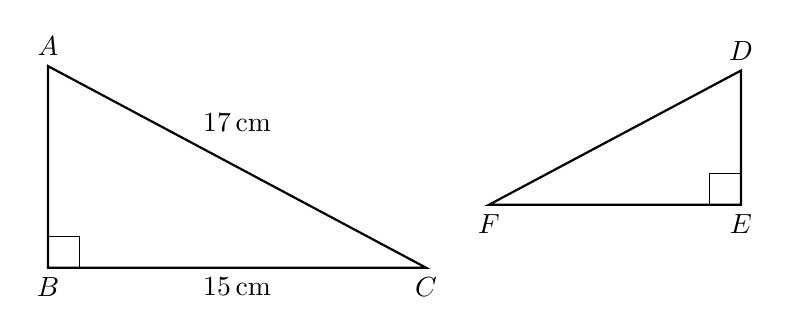
\begin{tikzpicture}[scale=0.8]
    \draw [thick]
      (0,0)node[below]{$F$}--
      (4,0)node[below]{$E$}--
      (4,2.13)node[above]{$D$}--cycle;
      \draw (4,0)++(-0.5,0)--++(0,0.5)--+(0.5,0);
    \draw [thick]
      (-1,-1)node[below]{$C$}--
      (-7,2.2)node[above]{$A$}--
      (-7,-1)node[below]{$B$}--cycle;
      \draw (-7,-1)++(0.5,0)--++(0,0.5)--+(-0.5,0);
      \node at (-4,-1)[below]{$15 \, \rm{cm}$};
      \node at (-4,1.3){$17 \, \rm{cm}$};
  \end{tikzpicture}
  \end{center}
If $\triangle ABC \sim \triangle DEF$, with right angles B and E, $BC=15$ cm, and $AC=17$ cm, what is the measure of $\angle F$, to the \emph{nearest degree}?

\item In triangle $MAH$ below, $\overline{MT}$ is the perpendicular bisector of $\overline{AH}$.
  \begin{center}
    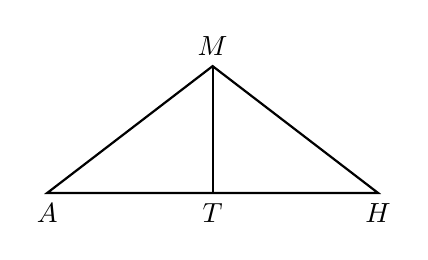
\begin{tikzpicture}[scale=0.7]
    \draw [thick]
    (0,0)node[below]{$A$}--
    (6,0)node[below]{$H$}--
    (3,2.3)node[above]{$M$}--cycle;
    \draw [thick](3,0)node[below]{$T$}--(3,2.3);
  \end{tikzpicture}
  \end{center}
Which statement is \emph{not} always true?
  \begin{enumerate}
    \item $\triangle MAH$ is isosceles.
    \item $\triangle MAT$ is isosceles.
    \item $\overline{MT}$ bisects $\angle AMH$.
    \item $\angle A$ and $\angle TMH$ are complementary.
  \end{enumerate}

\item In circle $B$ below, diameter $\overline{RT}$, radius $\overline{BE}$, and chord $\overline{RE}$ are drawn.
\begin{center}
  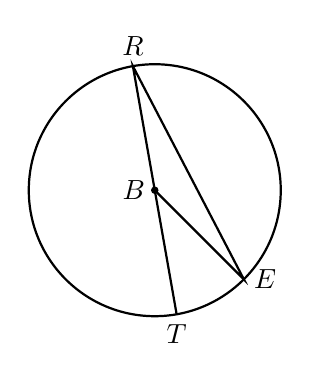
\begin{tikzpicture}[scale=0.8, rotate=0]
    \draw [thick] (0,0)--(100:2)node[above]{$R$}--
    (-45:2)node[right]{$E$}--cycle;
    \draw [thick] (0,0)--(-80:2)node[below]{$T$};
    \draw [fill] (0,0) circle [radius=0.05] node[left]{$B$};
    \draw [thick](0,0) circle [radius=2];
  \end{tikzpicture}
  \end{center}
  It $m\angle TRE = 15^\circ$ and $BE=9$, then the area of sector $EBR$ is what in terms of $\pi$?

\item Lou has a solid clay brick in the shape of a rectangular prism with a length of 8 inches, a width of 3.5 inches, and a height of 2.25 inches. If the clay weighs 1.055 oz/in$^3$, how much does Lou's brick weigh, to the nearest ounce? 

\item For the acute angles in a right triangle, $\sin (4x)^\circ =\cos (3x +13)^\circ$. \\
What is the number of degrees in the measure of the smaller angle?

\item A rectangular tabletop will be made of maple wood that weighs 43 pounds per cubic foot. The tabletop will have a length of eight feet, a width of three feet, and a thickness of one inch. Determine and state the weight of the tabletop, in pounds.

\item Determine and state an equation of the line perpendicular to the line\\ $5x-4y=10$ and passing through the point $(5,12)$.

\subsubsection*{Regents review and practice \hfill January 2019}
\item After a dilation with center $(0,0)$, the image of $\overline{DB}$ is $\overline{D'B'}$. If $DB=4.5$ and $D'B'=18$, then what is the scale factor of this dilation?

\item In the diagram below of circle $O$, points $K$, $A$, $T$, $I$, and $E$ are on the circle, $\triangle KAE$ and $\triangle ITE$ are drawn, $\wideparen{KE} \cong \wideparen{EI}$, and $\angle EKA \cong \angle EIT$.
\begin{center}
  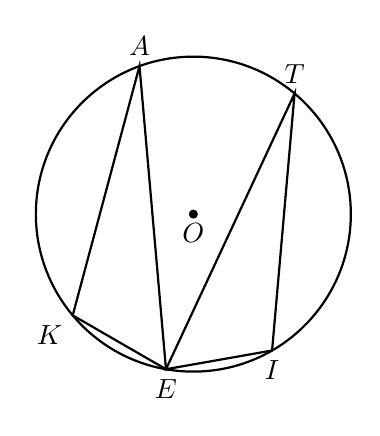
\begin{tikzpicture}[scale=1, rotate=0]
    \draw [fill] (0,0) circle [radius=0.05] node[below]{$O$};
    \draw [thick](0,0) circle [radius=2];
    \draw [thick] 
      (110:2)node[above]{$A$}--
      (220:2)node[below left]{$K$}--
      (-100:2)node[below]{$E$}--cycle;
    \draw [thick] 
      (50:2)node[above]{$T$}--
      (-60:2)node[below]{$I$}--
      (-100:2)--cycle;
  \end{tikzpicture}
  \end{center}
  Which statement about $\triangle KAE$ and $\triangle ITE$ is always true?
  \begin{enumerate}
    \item They are neither congruent nor similar.
    \item They are similar but not congruent.
    \item They are right triangles.
    \item They are congruent.
  \end{enumerate}

\item From a point on the ground one-half mile from the base of a historic monument, the angle of elevation to its top is $11.87^\circ$. To the nearest foot, what is the height of the monument? (1 mile = 5280 feet)

\item The area of a sector of a circle with a radius measuring 15 cm is $75\pi \; \rm{cm}^2$. What is the measure of the central angle that forms the sector?

\item Point $M$ divides $\overline{AB}$ so that $AM:MB = 1:2$. If $A$ has coordinates $(-1,-3)$ and $B$ has coordinates $(8,9)$, what are the coordinates of $M$?

\item What is an equation of the image of the line $\displaystyle y=\frac{3}{2}x-4$ after a dilation of a scale factor of $\displaystyle \frac{3}{4}$ centered at the origin?

\item Which three-dimensional figure will result when a rectangle 6 inches long and 5 inches wide is continuously rotated about the longer side?
\begin{enumerate}
  \item a rectangular prism with a length of 6 inches, width of 6 inches, and height of 5 inches
  \item a rectangular prism with a length of 6 inches, width of 5 inches, and height of 5 inches
  \item a cylinder with a radius of 5 inches and a height of 6 inches
  \item a cylinder with a radius of 6 inches and a height of 5 inches
\end{enumerate}

\item In the diagram below of triangle $ABC$, $\overline{AC}$ is extended through point $C$ to point $D$, and $\overline{BE}$ is drawn to $\overline{AC}$.
  \begin{center}
    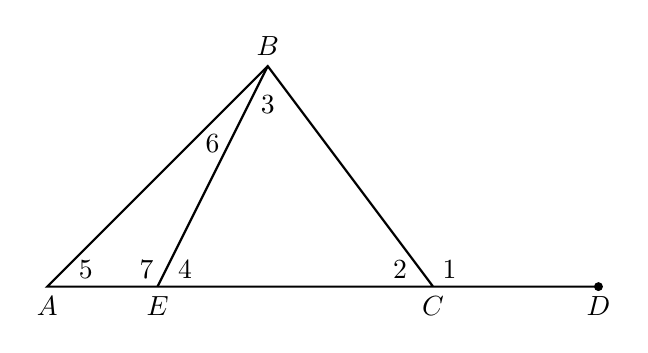
\begin{tikzpicture}[scale=0.7]
    \draw [thick]
    (10,0)node[below]{$D$}--
    (0,0)node[below]{$A$}--
    (4,4)node[above]{$B$}--
    (7,0)node[below]{$C$};
    \draw [fill] (10,0) circle [radius=0.07];
    \draw [thick](2,0)node[below]{$E$}--(4,4);
    \node at (0.7,0.3){5};
    \node at (1.8,0.3){7};
    \node at (2.5,0.3){4};
    \node at (6.4,0.3){2};
    \node at (7.3,0.3){1};
    \node at (3.0,2.6){6};
    \node at (4,3.3){3};
  \end{tikzpicture}
  \end{center}
Which equation is always true?
\begin{multicols}{2}
  \begin{enumerate}
    \item $\angle 1 = m\angle 3 + m\angle 2$
    \item $\angle 5 = m\angle 3 - m\angle 2$ 
    \item $\angle 6 = m\angle 3 - m\angle 2$
    \item $\angle 7 = m\angle 3 + m\angle 2$
  \end{enumerate}
\end{multicols}

\newpage
\item In right triangle $ABC$, $m\angle C=90^\circ$ and $AC \ne BC$. Which trigonometric ratio is equivalent to $\sin B$?
\begin{multicols}{2}
  \begin{enumerate}
    \item $\cos A$
    \item $\cos B$
    \item $\tan A$
    \item $\tan B$
  \end{enumerate}
\end{multicols}

\item In the diagram below of right triangle $ABC$, $AC=8$, and $AB=17$.
  \begin{center}
    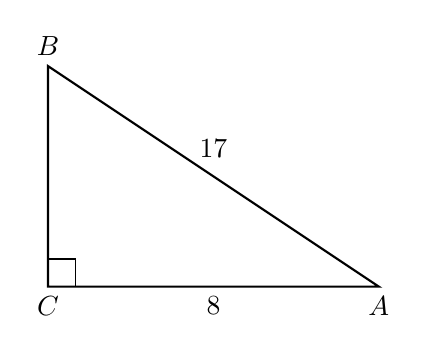
\begin{tikzpicture}[scale=0.7]
    \draw [thick]
      (0,0)node[below]{$A$}--
      (-6,4)node[above]{$B$}--
      (-6,0)node[below]{$C$}--cycle;
      \draw (-6,0)++(0.5,0)--++(0,0.5)--+(-0.5,0);
      \node at (-3,0)[below]{$8$};
      \node at (-3,2.5){$17$};
  \end{tikzpicture}
  \end{center}
Which equation would determine the value of angle $A$?
  \begin{multicols}{2}
    \begin{enumerate}
      \item $\displaystyle \sin A = \frac{8}{17}$
      \item $\displaystyle \tan A = \frac{8}{15}$
      \item $\displaystyle \cos A = \frac{15}{17}$
      \item $\displaystyle \tan A = \frac{15}{8}$
    \end{enumerate}
  \end{multicols}

\item Which equation represents a line that is perpendicular to the line represented by\\[0.25cm] $\displaystyle y=\frac{2}{3}x+1$?
  \begin{multicols}{2}
    \begin{enumerate}
      \item $3x+2y=12$
      \item $3x-2y=12$ 
      \item $\displaystyle y=\frac{3}{2}x+2$
      \item $\displaystyle y=-\frac{2}{3}x+4$
    \end{enumerate}
  \end{multicols}

\newpage
\item In diagram of quadrilateral $NAVY$, $m\angle YNA = 30^\circ$, $m\angle YAN = 38^\circ$,\\ $m\angle AVY = 94^\circ$, and $m\angle VAY = 46^\circ$.
\begin{center}
  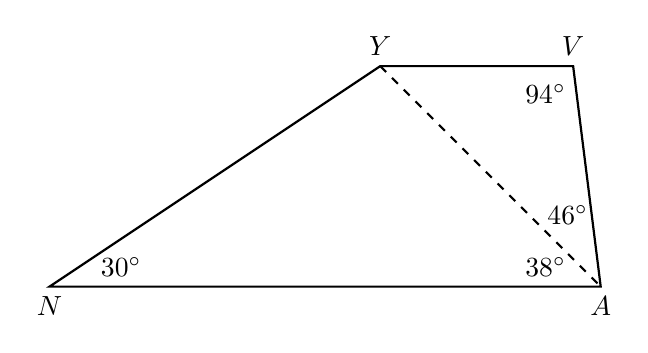
\begin{tikzpicture}[scale=0.7]
    \draw [thick] 
      (0,0)node[below]{$N$}--
      (10,0)node[below]{$A$}--
      (9.5,4)node[above]{$V$}--
      (6,4)node[above]{$Y$}--cycle;
    \draw [dashed, thick] (6,4)--(10,0);
    \node at (1.3,0.35){$30^\circ$};
    \node at (9,0.35){$38^\circ$};
    \node at (9.4,1.3){$46^\circ$};
    \node at (9,3.5){$94^\circ$};
  \end{tikzpicture}
  \end{center}
Which segment has the shortest length?
  \begin{multicols}{2}
  \begin{enumerate}
    \item $\overline{AY}$
    \item $\overline{NY}$
    \item $\overline{VA}$
    \item $\overline{VY}$
  \end{enumerate}
  \end{multicols}

\item In the diagram below, $\triangle ABC$, altitude $\overline{CG}$, and median $\overline{CM}$ are drawn.
\begin{center}
  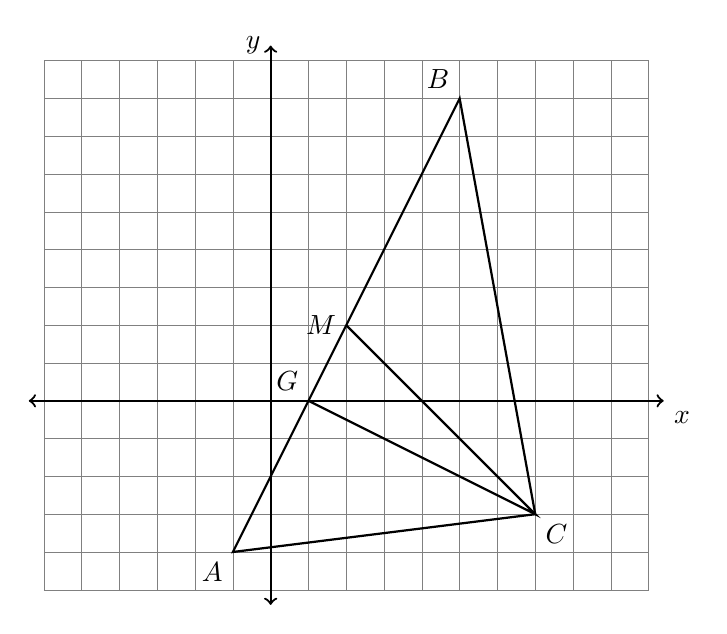
\begin{tikzpicture}[scale=.48]
    \draw [help lines] (-6,-5) grid (10,9);
    \draw [thick, <->] (-6.4,0) -- (10.4,0) node [below right] {$x$};
    \draw [thick, <->] (0,-5.4)--(0,9.4) node [left] {$y$};
    \draw [thick] 
      (-1,-4)node[below left]{$A$}--
      (7,-3)node[below right]{$C$}--
      (5,8)node[above left]{$B$}--cycle;
    \draw [thick] 
      (1,0)node[above left]{$G$}--
      (7,-3)--
      (2,2)node[left]{$M$};
  \end{tikzpicture}
\end{center}
Which expression represents the area of $\triangle ABC$?
  \begin{multicols}{2}
  \begin{enumerate}
    \item $\displaystyle \frac{(BC)(AC)}{2}$
    \item $\displaystyle \frac{(GC)(BC)}{2}$
    \item $\displaystyle \frac{(CM)(AB)}{2}$
    \item $\displaystyle \frac{(GC)(AB)}{2}$
  \end{enumerate}
  \end{multicols}

\newpage
\item As shown in the diagram below, the radius of a cone is 2.5 cm and its slant height is 6.5 cm.
  \begin{center}
    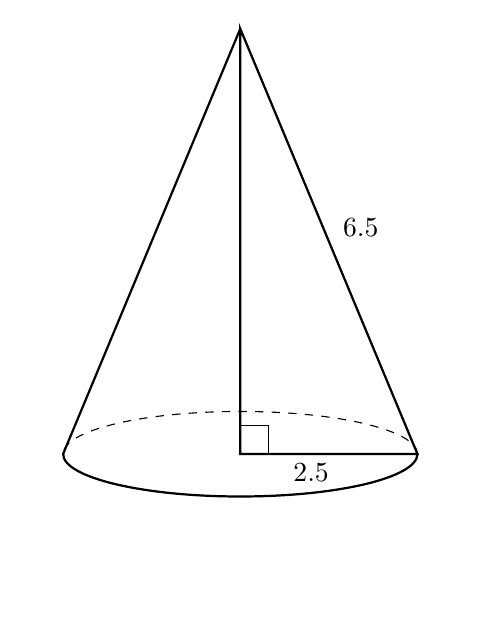
\begin{tikzpicture}[scale=0.9]
    \draw [thick] (0,0)--(2.5,0)--(0,6)--cycle;
    \draw (0,0)++(0.4,0)--++(0,0.4)--+(-0.4,0);
    \draw [thick] (0,6)--(-2.5,0);
    \node at (1,0)[below]{$2.5$};
    \node at (1.7,3.2){$6.5$};
    \draw [dashed] (0,0) ellipse [x radius=2.5,y radius=0.6];
    \clip (-3,-2) rectangle (3,0);
    \draw [thick] (0,0) ellipse [x radius=2.5,y radius=0.6];
  \end{tikzpicture}
  \end{center}
How many cubic centimeters are in the volume of the cone? Express your answer in terms of $\pi$.

\subsubsection*{Regents review and practice \hfill August 2018}
\item In the diagram below, $\overline{AEFB} \parallel \overline{CGD}$, and $\overline{GE}$ and $\overline{GF}$ are drawn.
\begin{center}
  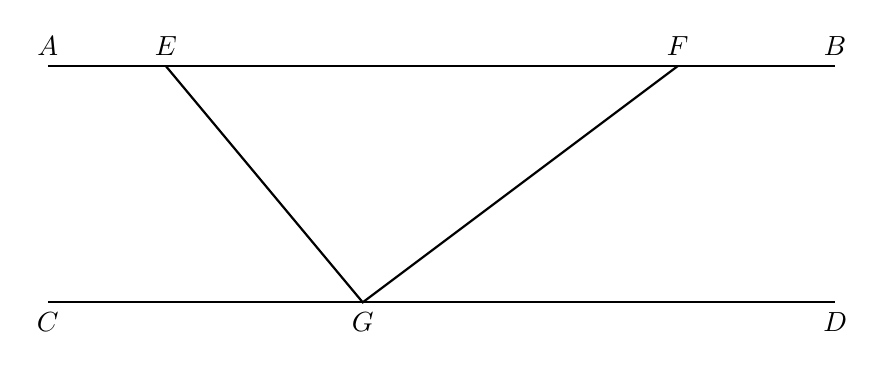
\begin{tikzpicture}[scale=1]
    \draw [thick] (0,0)node[below]{$C$}--(10,0)node[below]{$D$};
    \draw [thick] (0,3)node[above]{$A$}--(10,3)node[above]{$B$};
    \draw [thick] 
      (1.5,3)node[above]{$E$}--
      (4,0)node[below]{$G$}--
      (8,3)node[above]{$F$};
  \end{tikzpicture}
  \end{center}
If $m\angle EFG = 32^\circ$ and $m\angle AEG = 137^\circ$, what is $m\angle EGF$?
\begin{multicols}{2}
  \begin{enumerate}
    \item $11^\circ$
    \item $43^\circ$
    \item $75^\circ$
    \item $105^\circ$
  \end{enumerate}
\end{multicols}

\newpage
\item An isosceles right triangle whose legs measure 6 is continuously rotated about one of its legs to form a three-dimensional object. The three-dimensional object is a
  \begin{enumerate}
    \item cylinder with a diameter of 6
    \item cylinder with a diameter of 12
    \item cone with a diameter of 6
    \item cone with a diameter of 12
  \end{enumerate}

\item The coordinates of the endpoints of directed line segment $ABC$ are $A(-8,7)$ and $C(7,-13)$. If $AB:BC = 3:2$, what are the coordinates of $B$?

\item A circle with a diameter of 10 cm and a central angle of $30^\circ$ is drawn below.
\begin{center}
  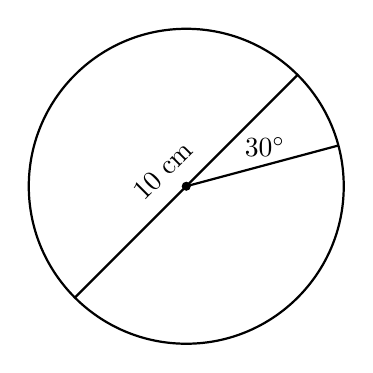
\begin{tikzpicture}[scale=1, rotate=0]
    \draw [thick] (45:2)--(225:2);
    \draw [thick] (0,0)--(15:2);
    \draw [fill] (0,0) circle [radius=0.05];
    \draw [thick](0,0) circle [radius=2];
    \node at (1,0.5){$30^\circ$};
    \node at (-0.3,0.2)[rotate=45]{$10 \; \rm{cm}$};
  \end{tikzpicture}
  \end{center}
  What is the area, to the \emph{nearest tenth of a square centimeter}, of the sector formed by the $30^\circ$ angle?

\item A child's tent can be modeled as a pyramid with a square base whose sides measure 60 inches and whose height measures 84 inches. What
is the volume of the tent, to the \emph{nearest cubic foot}?

\subsubsection*{Regents review and practice \hfill August 2018}
\item Given square $RSTV$, where $RS=9$ cm. If square $RSTV$ is dilated by a scale factor of 3 about a given center, what is the perimeter, in centimeters, of the image of $RSTV$ after the dilation?

\item In right triangle $ABC$, hypotenuse $\overline{AB}$ has a length of 26 cm, and side $\overline{BC}$ has a length of 17.6 cm. What is the measure of angle $B$, to the \emph{nearest degree}?

\item In a right triangle, the acute angles have the relationship \\$\sin (2x + 4)=\cos (46)$.\\[0.25cm]
What is the value of $x$?

\item The base of a pyramid is a rectangle with a width of 4.6 cm and a
length of 9 cm. What is the height, in centimeters, of the pyramid if
its volume is 82.8 cm$^3$?

\item What is an equation of the line that passes through the point $(6,8)$
and is perpendicular to a line with equation $y=\frac{3}{2}x+5$?
  \begin{multicols}{2}
    \begin{enumerate}
      \item $y-8=\frac{3}{2}(x-6)$
      \item $y-8=-\frac{3}{2}(x-6)$ 
      \item $y+8=\frac{3}{2}(x+6)$
      \item $y+8=-\frac{3}{2}(x+6)$
    \end{enumerate}
  \end{multicols}

\item Directed line segment $DE$ has endpoints $D(-4, -2)$ and $E(1,8)$.
Point $F$ divides such that $DF:FE$ is $2:3$. What are the coordinates
of $F$?

\item Line segment $CD$ is the altitude drawn to hypotenuse in right
triangle $ECF$. If $EC=10$ and $EF=24$, then, to the \emph{nearest
tenth}, $ED$ is what length?

\item Line $MN$ is dilated by a scale factor of 2 centered at the point $(0,6)$. If $\overline{MN}$ is represented by $y=-3x+6$, which equation can represent $\overline{M'N'}$, the image of $\overline{MN}$?
  \begin{multicols}{2}
    \begin{enumerate}
      \item $y=-3x+12$
      \item $y=-3x+6$ 
      \item $y=-6x+12$
      \item $y=-6x+6$
    \end{enumerate}
  \end{multicols}

\item Triangle $A'B'C'$ is the image of triangle $ABC$ after a translation of 2 units to the right and 3 units up. Is triangle $ABC$ congruent to triangle $A'B'C'$? Explain why.

\item Randy's basketball is in the shape of a sphere with a maximum circumference of 29.5 inches. Determine and state the volume of the basketball, to the \emph{nearest cubic inch}.

\end{enumerate}
\end{document}
